\section{Areas in Polar Coordinates}\label{sec:Areas in polar coordinates}
We can use the equation of a curve in polar coordinates to compute
some areas bounded by such curves.
The basic approach is the same as with any application of integration:
Find an approximation that approaches the true value. For areas in
rectangular coordinates, we approximated the region using rectangles;
in polar coordinates, we use sectors of circles, as depicted in
Figure~\ref{fig:approximating area with sectors}. Recall that the
area of a sector of a circle is $\ds \alpha r^2/2$, where $\alpha$ is the
angle subtended by the sector. If the curve is given by $r=f(\theta)$,
and the angle subtended by a small sector is $\Delta\theta$, 
the area is $\ds (\Delta\theta)(f(\theta))^2/2$.
Thus we approximate the total area as
$$\sum_{i=0}^{n-1} {1\over 2} f(\theta_i)^2\;\Delta\theta.$$
As a limit, this will give rise to:
$$\int_a^b {1\over 2} f(\theta)^2\;d\theta.$$

\begin{example}{Area inside a Cardioid}{cardioidarea}
Find the area inside the cardioid $r=1+\cos\theta$.
\end{example}

\begin{solution}
$$\int_0^{2\pi}{1\over 2} (1+\cos\theta)^2\;d\theta=
\ds{1\over 2}\int_0^{2\pi} 1+2\cos\theta+\cos^2\theta\;d\theta=
\ds{1\over 2}\left(\theta +2\sin\theta+
\ds{\theta\over2}+\ds{\sin2\theta\over4}\middle)\right|_0^{2\pi}={3\pi\over2}.$$
\end{solution}

As in the example above, if a function is defined over the complete region $[0,2\pi]$, then the bounds for the integral are $a=0$, $b=2\pi$. However, sometimes we need to be careful!

\begin{example}{Area inside a Loop}{areainloop}
Find the area inside the loop $r=\sqrt{\cos\theta}$.
\end{example}
\begin{solution}
We look for points of intersection.
\begin{align*}
0&=\sqrt{\cos\theta}	\\
0&=\cos\theta
\end{align*}
This has solutions $\theta=\pi/2$ and $3\pi/2$, but we must select our bounds for integration correctly. Since $\cos\theta$ is negative on $(\pi/2,3\pi/3)$, $\sqrt{\cos\theta}$ is undefined. Note that one full revolution is $2\pi$; that is, the function is $2\pi$ periodic. If we were to integrate on $[3\pi/2,\pi/2]$ we would get the same answer, and can avoid a scenario in which $\sqrt{\cos\theta}$ is undefined. Equivalently, we can integrate on $[-\pi/2,\pi/2]$.
\[\ds \int_a^b\frac{1}{2} f(\theta)^2\,d\theta=\int_{-\pi/2}^{\pi/2}\frac{1}{2}\left(\sqrt{\cos\theta}\right)^2\,d\theta=\frac{1}{2}\int_{-\pi/2}^{\pi/2}\cos\theta\,d\theta=\frac{1}{2}\Big(\sin\theta\Big)\Big|_{-\pi/2}^{\pi/2}=1\]
\end{solution}

\figure[H]
\centerline{\vbox{\beginpicture
\normalgraphs
%\ninepoint
\setcoordinatesystem units <20truemm,20truemm>
\setplotarea x from 0 to 2.5, y from 0  to 1.5
\axis left shiftedto x=0 /
\axis bottom shiftedto y=0 /
\setquadratic
\plot 1.941 0.393 1.900 0.506 1.850 0.613 1.791 0.715 1.723 0.811
1.648 0.900 1.565 0.981 1.476 1.054 1.382 1.118 1.284 1.172
1.182 1.217 1.078 1.252 0.973 1.278 0.867 1.293 0.762 1.299
0.659 1.295 0.559 1.283 0.462 1.262 0.369 1.233 0.281 1.196
0.199 1.153 /
\setlinear
\plot 0 0 0.75 1.299 /
\circulararc -15 degrees from 0.75 1.299 center at 0 0 
\plot 0 0 1.207 1.207 /
\circulararc -15 degrees from 1.207 1.207 center at 0 0
\plot 0 0 1.616 0.933 / 
\circulararc -15 degrees from 1.616 0.933 center at 0 0
\plot 0 0 1.9 0.51 /
\endpicture}}
\caption{{Approximating area by sectors of circles.} \label{fig:approximating area with sectors}}
\endfigure

\begin{example}{Area Between Circles}{areabetweencircles}
Find the area between the circles $r=2$ and
$r=4\sin\theta$, as shown in figure~\ref{fig:polar area between curves}.
\end{example}

\begin{solution}
The two curves intersect where $2=4\sin\theta$, or $\sin\theta=1/2$,
so $\theta=\pi/6$ or $5\pi/6$. The area we want is then
$$
  {1\over2}\int_{\pi/6}^{5\pi/6}
  16\sin^2\theta-4\;d\theta={4\over3}\pi + 2\sqrt{3}.
$$
\end{solution}

%\figure[!ht]
%\centerline{
%\hbox{\hfill\tikzpicture[domain=-2:2,x=6mm,y=6mm]
%\draw[->] (-2.1,0) -- (2.1,0) ;
%\draw[->] (0,-2.1) -- (0,4.1) ;
%\gpad
%\draw[color=black] plot[parametric,id=\the\gpnum,domain=0:2*3.1416,samples=50] 
%function{2*cos(t),2*sin(t)};
%\gpad
%\draw[color=black] plot[parametric,id=\the\gpnum,domain=0:3.1416,samples=50] 
%function{4*sin(t)*cos(t),4*sin(t)*sin(t)};
%\gpad
%\fill[opacity=0.5,fill=red!20] 
%plot[parametric,id=\the\gpnum,domain=0.5236:2.618]
%function{4*sin(t)*cos(t),4*sin(t)*sin(t)} node {\gpad}
%plot[parametric,id=\the\gpnum,domain=0.5236:2.618]
%function{2*cos(3.1416-t),2*sin(3.1416-t)} -- cycle;
%\endtikzpicture\hfill}}
%\caption{{An area between curves.} \label{fig:polar area between curves}}
%\endfigure

\figure[H]
\[
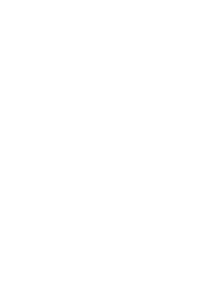
\includegraphics[width=1.75in]{images/7-area-circles} 
\] 
\caption{{An area between curves.} \label{fig:polar area between curves}}
\endfigure

This first example makes the process appear more straightforward than it
is. Since points have many different representations in polar
coordinates, it is not always so easy to identify points of
intersection. 

\begin{example}{Shaded Area}{shadedarea}
Find the shaded area in the first graph of
figure~\ref{fig:harder area between polar curves} as the difference
of the other two shaded areas. The cardioid is $r=1+\sin\theta$ and
the circle is $r=3\sin\theta$. 
\end{example}

\begin{solution}
We attempt to find points of intersection:
\begin{eqnarray*}
  1+\sin\theta&=3\sin\theta\cr
  1&=2\sin\theta\cr
  1/2&=\sin\theta.\cr
\end{eqnarray*}
This has solutions $\theta=\pi/6$ and $5\pi/6$; $\pi/6$ corresponds to
the intersection in the first quadrant that we need.  Note that no
solution of this equation corresponds to the intersection point at the
origin, but fortunately that one is obvious. The cardioid goes through
the origin when $\theta=-\pi/2$; the circle goes through the origin at
multiples of $\pi$, starting with $0$.

Now the larger region has area
$$
  {1\over2}\int_{-\pi/2}^{\pi/6} (1+\sin\theta)^2\;d\theta=
  {\pi\over2}-{9\over16}\sqrt{3},
$$
and the smaller has area
$$
  {1\over2}\int_{0}^{\pi/6} (3\sin\theta)^2\;d\theta=
  {3\pi\over8} - {9\over16}\sqrt{3},
$$
so the difference is the area we seek, which is $\pi/8$.
\end{solution}



%\figure[!ht]
%\centerline{
%\hbox to \hsize{\hfill\tikzpicture[domain=-2:2,x=9mm,y=9mm]
%\draw[->] (-1.6,0) -- (1.6,0) ;
%\draw[->] (0,-1) -- (0,3.1) ;
%\gpad
%\draw[color=black] plot[parametric,id=\the\gpnum,domain=0:2*pi,samples=50] 
%function{(1+sin(t))*cos(t),(1+sin(t))*sin(t)};
%\gpad
%\draw[color=black] plot[parametric,id=\the\gpnum,domain=0:pi,samples=50] 
%function{3*sin(t)*cos(t),3*sin(t)*sin(t)};
%\gpad
%\fill[opacity=0.5,fill=red!20] 
%plot[parametric,id=\the\gpnum,domain=-pi/2:pi/6]
%function{(1+sin(t))*cos(t),(1+sin(t))*sin(t)} node {\gpad}
%plot[parametric,id=\the\gpnum,domain=0:pi/6] 
%function{3*sin(pi/6-t)*cos(pi/6-t),3*sin(pi/6-t)*sin(pi/6-t)}; 
%\endtikzpicture
%\quad
%\tikzpicture[domain=-2:2,x=9mm,y=9mm]
%\draw[->] (-1.6,0) -- (1.6,0) ;
%\draw[->] (0,-1) -- (0,3.1) ;
%\gpad
%\draw[color=black] plot[parametric,id=\the\gpnum,domain=0:2*pi,samples=50] 
%function{(1+sin(t))*cos(t),(1+sin(t))*sin(t)};
%\gpad
%\draw[color=black] plot[parametric,id=\the\gpnum,domain=0:pi,samples=50] 
%function{3*sin(t)*cos(t),3*sin(t)*sin(t)};
%\gpad
%\fill[opacity=0.5,fill=red!20] 
%plot[parametric,id=\the\gpnum,domain=-pi/2:pi/6]
%function{(1+sin(t))*cos(t),(1+sin(t))*sin(t)}; 
%\endtikzpicture
%\quad
%\tikzpicture[domain=-2:2,x=9mm,y=9mm]
%\draw[->] (-1.6,0) -- (1.6,0) ;
%\draw[->] (0,-1) -- (0,3.1) ;
%\gpad
%\draw[color=black] plot[parametric,id=\the\gpnum,domain=0:2*pi,samples=50] 
%function{(1+sin(t))*cos(t),(1+sin(t))*sin(t)};
%\gpad
%\draw[color=black] plot[parametric,id=\the\gpnum,domain=0:pi,samples=50] 
%function{3*sin(t)*cos(t),3*sin(t)*sin(t)};
%\gpad
%\fill[opacity=0.5,fill=red!20] 
%plot[parametric,id=\the\gpnum,domain=0:pi/6] 
%function{3*sin(t)*cos(t),3*sin(t)*sin(t)}; 
%\endtikzpicture
%\hfill}}
%\caption{{An area between curves.} \label{fig:harder area between polar curves}}
%\endfigure
\figure[H]
\[
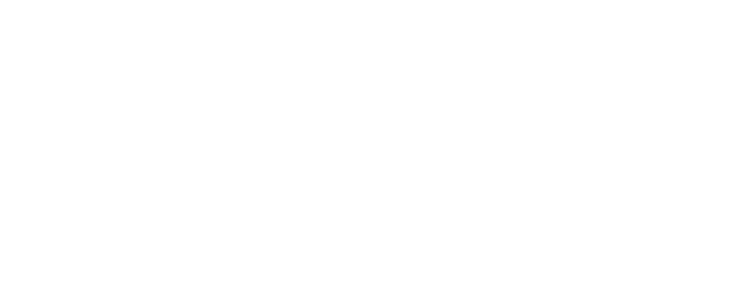
\includegraphics[width=4.5in]{images/7-area-between} 
\] 
\caption{{An area between curves.} \label{fig:harder area between polar curves}}
\endfigure


%%%%%%%%%%%%%%%%%%%%%%%%%%%%%%%%%%%%%%%%%%%%
\Opensolutionfile{solutions}[ex]
\section*{Exercises for \ref{sec:Areas in polar coordinates}}

\begin{enumialphparenastyle}

%%%%%%%%%%
\begin{ex}
Find the area enclosed by the curve.
\begin{multicols}{2}
\begin{enumerate}
	\item	$\ds r=\sqrt{\sin\theta}$
	\item	$\ds r=2+\cos\theta$
	\item	$\ds r=\sec\theta, \pi/6\le\theta\le\pi/3$
	\item	$\ds r=\cos\theta, 0\le\theta\le\pi/3$
	\item	$\ds r=2a\cos\theta, a>0$
	\item	$\ds r=4+3\sin\theta$
\end{enumerate}
\end{multicols}
\begin{sol}
\begin{multicols}{2}
\begin{enumerate}
	\item	$1$
	\item	$9\pi/2$
	\item	$\ds \sqrt3/3$
	\item	$\ds \pi/12+\sqrt3/16$
	\item	$\ds \pi a^2/4$
	\item	$41\pi/2$
\end{enumerate}
\end{multicols}
\end{sol}
\end{ex}

%%%%%%%%%%
\begin{ex}
 Find the area inside the loop formed by
$\ds r=\tan(\theta/2)$.
\begin{sol}
 $2-\pi/2$
\end{sol}
\end{ex}

%%%%%%%%%%
\begin{ex}
 Find the area inside one loop of $\ds r=\cos(3\theta)$.
\begin{sol}
 $\pi/12$
\end{sol}
\end{ex}

%%%%%%%%%%
\begin{ex}
 Find the area inside one loop of $\ds r=\sin^2\theta$.
\begin{sol}
 $3\pi/16$
\end{sol}
\end{ex}

%%%%%%%%%%
\begin{ex}
 Find the area inside the small loop of $\ds r=(1/2)+\cos\theta$.
\begin{sol}
 $\ds \pi/4-3\sqrt3/8$
\end{sol}
\end{ex}

%%%%%%%%%%
\begin{ex}
 Find the area inside $\ds r=(1/2)+\cos\theta$, including the
area inside the small loop.
\begin{sol}
 $\ds \pi/2+3\sqrt3/8$
\end{sol}
\end{ex}

%%%%%%%%%%
\begin{ex}
 Find the area inside one loop of $\ds r^2=\cos(2\theta)$.
\begin{sol}
 $1$
\end{sol}
\end{ex}

%%%%%%%%%%
\begin{ex}
 Find the area enclosed by $r=\tan\theta$ and 
$\ds r={\csc\theta\over\sqrt2}$.
\begin{sol}
 $3/2-\pi/4$
\end{sol}
\end{ex}

%%%%%%%%%%
\begin{ex}
 Find the area inside $r=2\cos\theta$ and outside
$r=1$.
\begin{sol}
 $\ds \pi/3+\sqrt3/2$
\end{sol}
\end{ex}

%%%%%%%%%%
\begin{ex}
 Find the area inside $r=2\sin\theta$ and above
the line $r=(3/2)\csc\theta$.
\begin{sol}
 $\ds \pi/3-\sqrt3/4$
\end{sol}
\end{ex}

%%%%%%%%%%
\begin{ex}
 Find the area inside $r=\theta$, $0\le\theta\le2\pi$.
\begin{sol}
 $\ds 4\pi^3/3$
\end{sol}
\end{ex}

%%%%%%%%%%
\begin{ex}
 Find the area inside $\ds r=\sqrt{\theta}$, $0\le\theta\le2\pi$.
\begin{sol}
 $\ds \pi^2$
\end{sol}
\end{ex}

%%%%%%%%%%
\begin{ex}
 Find the area inside both $\ds r=\sqrt3\cos\theta$ and
$r=\sin\theta$.
\begin{sol}
 $\ds 5\pi/24-\sqrt3/4$
\end{sol}
\end{ex}

%%%%%%%%%%
\begin{ex}
 Find the area inside both $r=1-\cos\theta$
and $r=\cos\theta$.
\begin{sol}
 $\ds 7\pi/12-\sqrt3$
\end{sol}
\end{ex}

%%%%%%%%%%
\begin{ex}
 The center of a circle of radius 1 is on the 
circumference of a circle of radius 2. Find the area 
of the region inside both circles.
\begin{sol}
 $\ds 4\pi-\sqrt{15}/2-7\arccos(1/4)$
\end{sol}
\end{ex}

%%%%%%%%%%
\begin{ex}
 Find the shaded area in figure~\ref{fig:area inside spiral}. 
The curve is $r=\theta$, $0\le\theta\le3\pi$.
\begin{sol}
 $\ds 3\pi^3$
\end{sol}
\end{ex}


%\figure[!ht]
%\centerline{
%\hbox to \hsize{\hfill
%\tikzpicture[domain=-2:2,x=4mm,y=4mm]
%\draw[->] (-10,0) -- (7,0) ;
%\draw[->] (0,-5.2) -- (0,8.5) ;
%\gpad
%\draw[color=black] plot[parametric,id=\the\gpnum,domain=0:3*pi,samples=100] 
%function{(t)*cos(t),(t)*sin(t)};
%\gpad
%\fill[opacity=0.5,fill=red!20] (0,0) -- (2*pi,0)
%plot[parametric,id=\the\gpnum,domain=2*pi:3*pi]
%function{(t)*cos(t),(t)*sin(t)} node {\gpad} -- (-pi,0)
%plot[parametric,id=\the\gpnum,domain=0:pi] 
%function{(pi-t)*cos(pi-t),(pi-t)*sin(pi-t)}; 
%\endtikzpicture
%\hfill}}
%\caption{{An area bounded by the spiral of Archimedes.} \label{fig:area inside spiral}}
%\endfigure
\figure[H]
\[
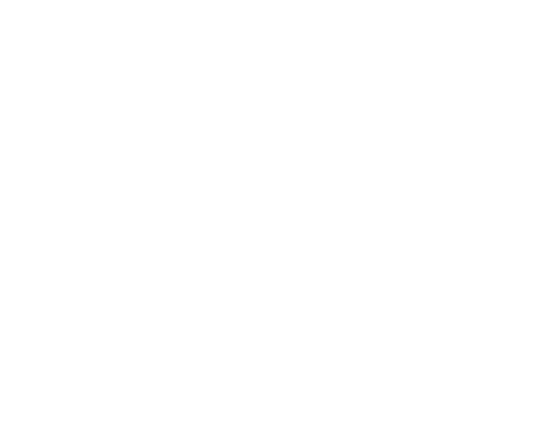
\includegraphics[width=2.75in]{images/7-arch} 
\] 
\caption{{An area bounded by the spiral of Archimedes.} \label{fig:area inside spiral}}
\endfigure

\end{enumialphparenastyle}